\section{Particle Identification by $dE/dx$}\label{sec:pid}
The specific ionization energy loss, the $dE/dx$, is a function of the
particle momentum magnitude. This property is used
for particle identification. This analysis focuses on particle
identification in the low $p_T$ region. This section describes
the low $p_T$ $dE/dx$ particle identification method in detail.
Extension of particle identification to high $p_T$ is possible
by the Time of Flight (TOF), $t^{TOF}=t^{stop}-t^{start}$ . Due to the low particle multiplicity and lack of signal in VPDs on the outgoing proton side (rapidity gap) in SD events, the $t^{start}$ is not defined precisely. Since that, the analysis was limited to identification only by $dE/dx$. \newline
The ionization energy loss by charged particles in material
is given by the Bethe-Bloch formula and for
thin material by the more precise Bichsel formula\cite{Bichsel:2006cs}.
With the measured particle momentum and $dE/dx$,
the particle type can be determined by comparing the
measurements against the Bethe-Bloch (Bichsel) expectation. Figure \ref{fig:dedx} shows the measured $dE/dx$ versus rigidity $q\times p$ for particles in $|\eta| < 0.7$. Various bands, corresponding
to different mass particles, are clearly separated
at low $|q\times p|$. At modest $|q\times p|$, the bands start to
overlap: $e^\pm$ and $K^\pm$ merge at $\sim0.4$~GeV/c, $K^\pm$ and
$\pi^\pm$ merge at $\sim0.7$~GeV/c, and $p(\bar{p})$ and $\pi^\pm$ merge
at $\sim1.1$~GeV/c. However, particles can still be statistically
identified by a fitting procedure. The
separation of the $dE/dx$ bands depends on the pseudorapidity
region and decreases toward higher rapidities.
In the midrapidity region of $|\eta| < 0.7$, $p_T$ is approximately equal to $|p|$.


\begin{figure}[H]
	\centering
	\parbox{0.99\textwidth}{
		\centering
		\begin{subfigure}[b]{\linewidth}{
				{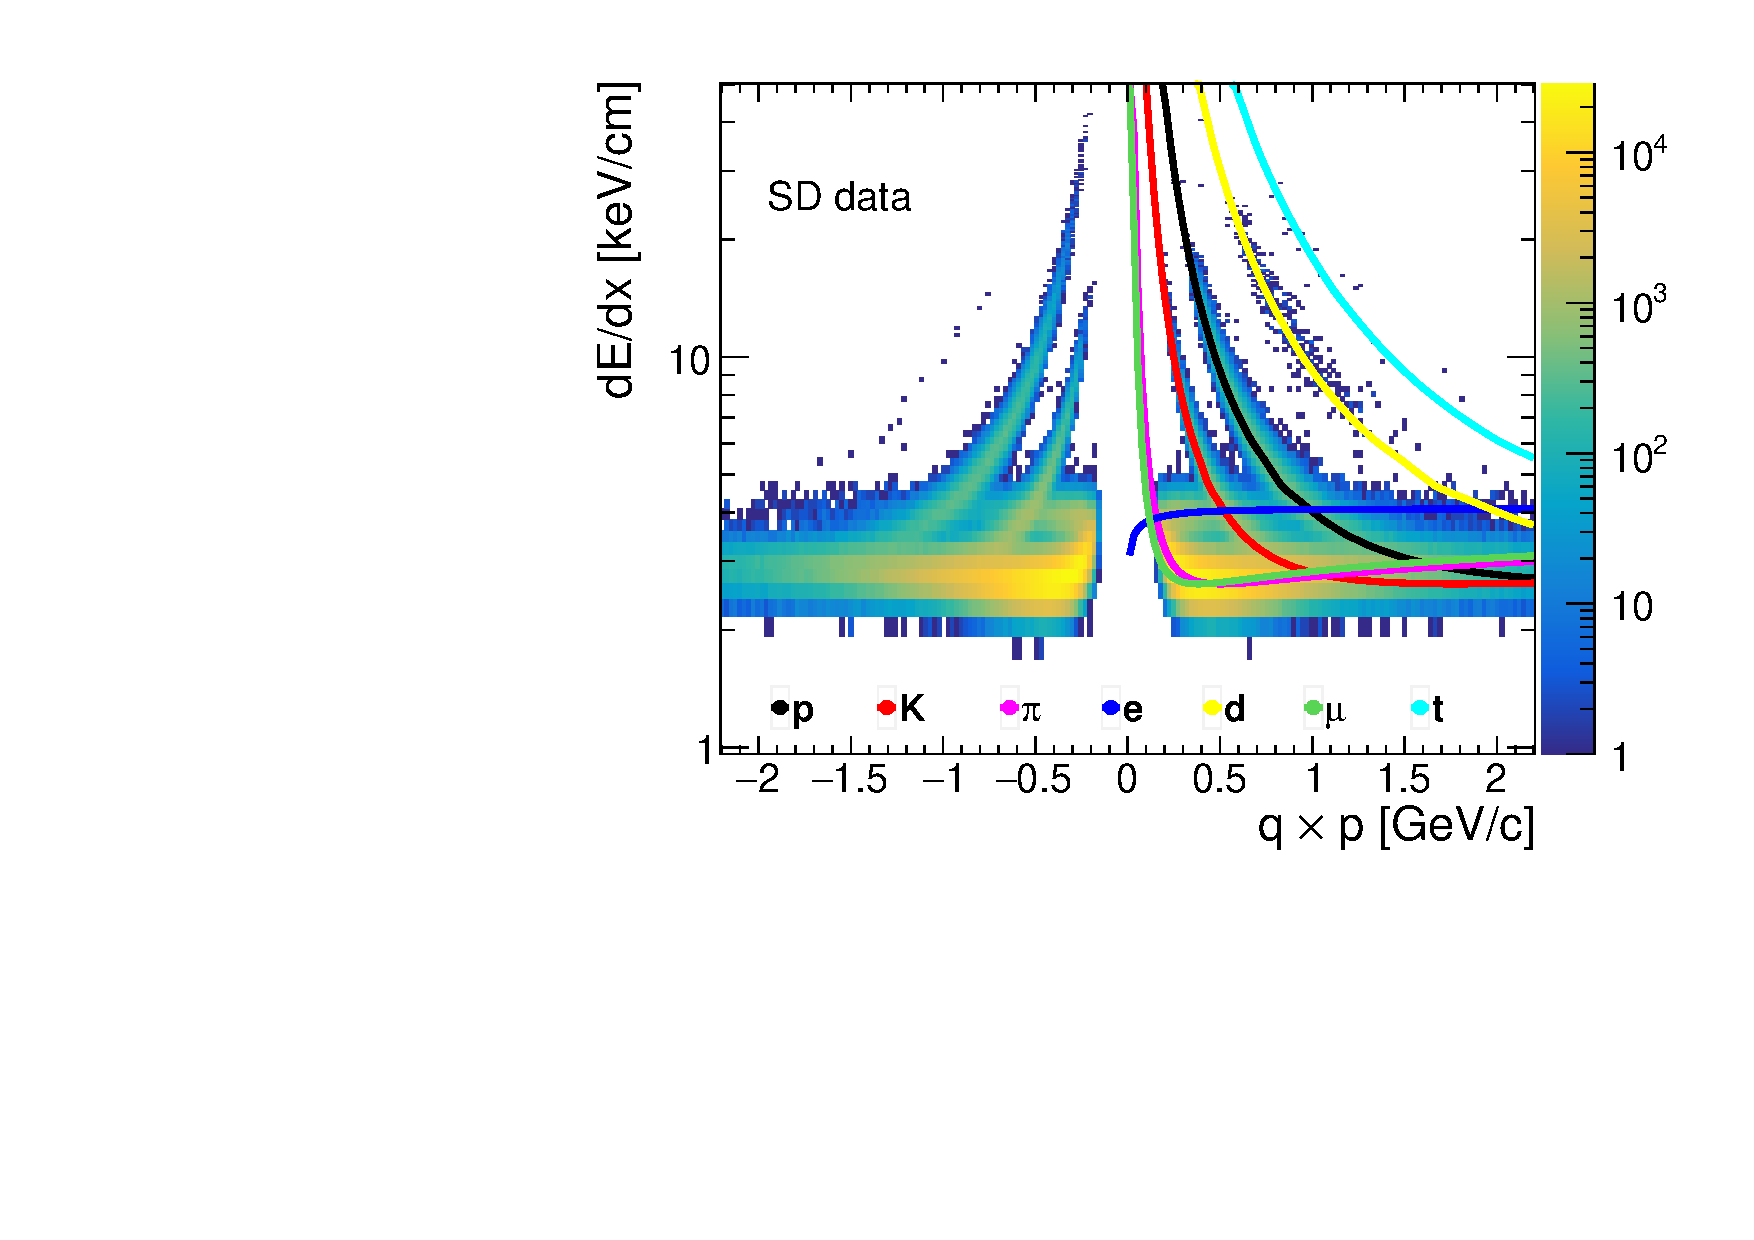
\includegraphics[width=\linewidth, page=1]{graphics/pid/SDT_dEdx.pdf}}}
		\end{subfigure}
	}
	\caption[Specific ionization
		energy loss $dE/dx$ as a function of rigidity $q\times p$ for particles
		in $|\eta| < 0.7$ measured in $200$~GeV SD pp collisions
		by the STAR-TPC]{Specific ionization
	energy loss $dE/dx$ as a function of rigidity $q\times p$ for particles
	in $|\eta| < 0.7$ measured in $200$~GeV SD pp collisions
	by the STAR-TPC. The Bichsel predictions for each particle species are also shown.}
	\label{fig:dedx}
\end{figure} 
\noindent Since the $dE/dx$ distribution for a fixed particle type
is not Gaussian, a new variable is useful in order
to have a proper deconvolution into Gaussians. A better Gaussian variable, for a given
particle type, is the $n\sigma^i_{dE/dx}$-variable, defined as
\begin{equation}
n\sigma^i_{dE/dx}=\ln\left(\frac{dE/dx}{(dE/dx)_i^{BB}}\right)/\sigma
\end{equation}
where $(dE/dx)_i^{BB}$ is the Bethe-Bloch (Bichsel) expectation
of $dE/dx$ for the given particle type $i (i =
\pi, K, p)$, $\sigma$ - the $dE/dx$ resolution.
The expected value of $n\sigma^i_{dE/dx}$ for the particle in study is around $0$  and the width equals to $1$. The $n\sigma^i_{dE/dx}$ is shown for $\pi^{\pm}$, $K^\pm$ and $p(\bar{p})$ in Fig.~\ref{fig:nsigma}.


\begin{figure}[H]
	\centering
	\parbox{0.484\textwidth}{
		\centering
		\begin{subfigure}[b]{\linewidth}{
				\subcaptionbox{\label{fig:nsigmaa}}{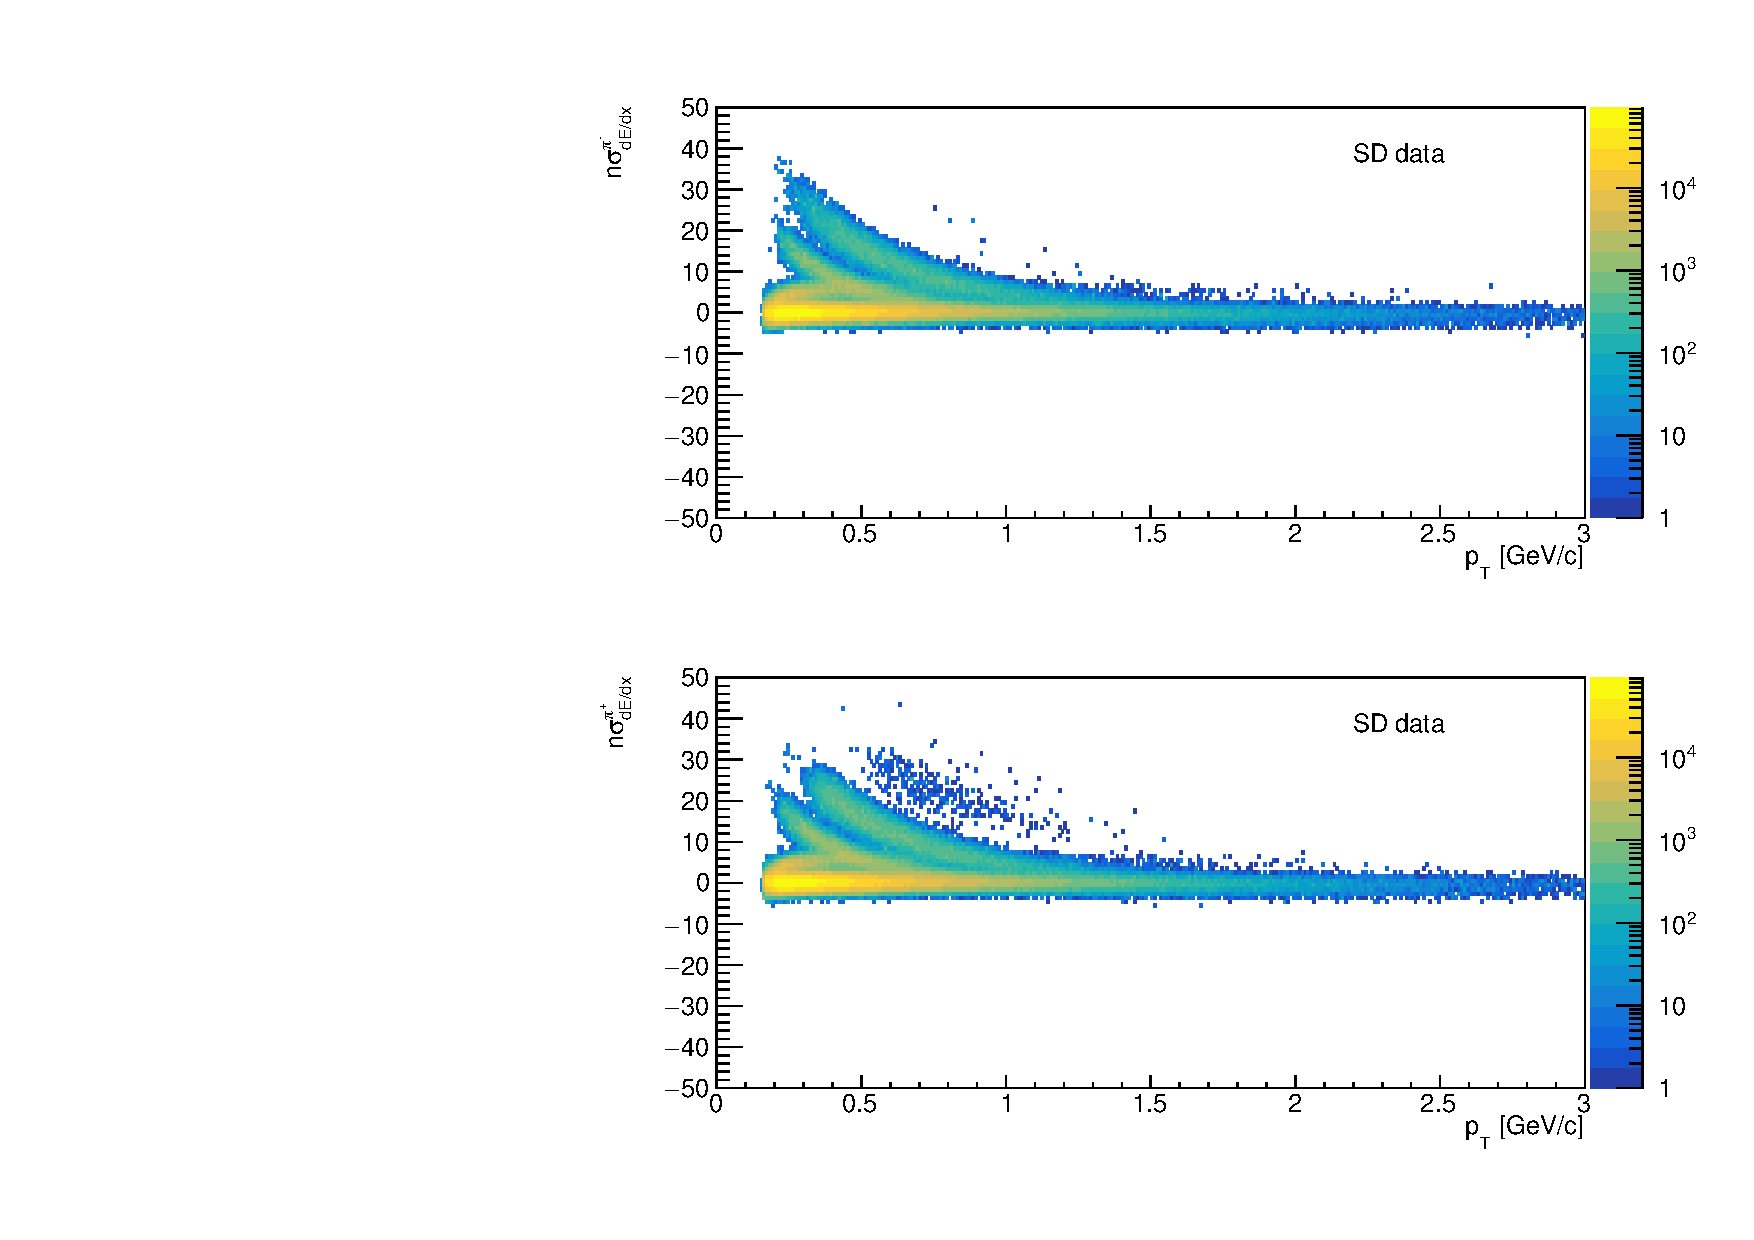
\includegraphics[width=\linewidth, page=1]{graphics/pid/spectraFit_SDT.pdf}}}
		\end{subfigure}
	}
	\quad
	\parbox{0.484\textwidth}{
		\centering
		\begin{subfigure}[b]{\linewidth}{
				\subcaptionbox{\label{fig:nsigmab}}{\includegraphics[width=\linewidth, page=14]{graphics/pid/spectraFit_SDT.pdf}}}
		\end{subfigure}
	}
	\parbox{0.484\textwidth}{
			\centering
			\begin{subfigure}[b]{\linewidth}{
					\subcaptionbox{\label{fig:nsigmac}}{\includegraphics[width=\linewidth, page=21]{graphics/pid/spectraFit_SDT.pdf}}}
			\end{subfigure}
		}
	\caption[The $n\sigma^{i}_{dE/dx}$ variable versus $p_T$ in SD collisions]{The $n\sigma^{i}_{dE/dx}$ variable for particle $i$, where $i=\pi^\pm, K^\pm, p/\bar{p}$, versus $p_T$ in SD collisions. Particles are restricted in $|\eta| < 0.7$
		and corrected for the energy loss (mass of $i$-particle was taken) and vertexing. In
		this narrow pseudorapidity slice, $p_T$ is approximately
		equal to $|p|$.}
	\label{fig:nsigma}
\end{figure}
\noindent Figure \ref{fig:nsigmafit}
shows the $n\sigma^{\pi^\pm}_{dE/dx}$,$n\sigma^{K^\pm}_{dE/dx}$ and $n\sigma^{p(\bar{p})}_{dE/dx}$ distributions for one $p_T$ bin, each corrected for the energy loss\cite{commonnote} (mass of $i$-particle was taken) and vertexing (other $p_T$ bins are shown in Appendix~\ref{appendix:dEdxFits}). To extract the  particle yield for a given particle type,
a~multi-Gaussian fit is applied to the $n\sigma^i_{dE/dx}$ distribution as
shown in Fig.~\ref{fig:nsigmafit}. The parameters of the multi-Gaussian fit are the centroids $\mu_{i^-/i^+}$, widths $\sigma_{i^-/i^+}$, sum  and ratios  of amplitudes $C_{i^-/i^+}$, $r_{i^-/i^+}$ for negative $i^-$ and positive $i^+$ particles ($\pi^\pm$, $e^\pm$, $K^\pm$, $p$ and $\bar{p}$). The positive and negative particle
$n\sigma^{i}_{dE/dx}$-distributions are fit simultaneously. The particle
and antiparticle centroids and widths are kept the same. Additionally, there are some assumptions depending on particle under study:
\begin{enumerate}
	\item $\pi^\pm$ fit:
	\begin{itemize}
		\item $p_T>0.35$~GeV/c: $r_{e^-/e^+}$ and $C_{e^-/e^+}$ are fixed to the MC prediction and scaled by the ratio of the fit result in bin with $0.3 < p_T < 0.35$~GeV/c to the MC prediction in that bin.
		\item $p_T>0.4$~GeV/c: electron width $\sigma_{e^-/e^+}$ is extrapolated from the lower-$p_T$ bins and fixed.
		\item $p_T>0.55$~GeV/c: kaon width $\sigma_{K^-/K^+}$ is extrapolated from the lower-$p_T$ bins and fixed.
		\item $p_T>0.75$~GeV/c: proton width $\sigma_{\bar{p}/p}$ is extrapolated from the lower-$p_T$ bins and fixed.
	\end{itemize}
	\item $K^\pm$ fit:
	\begin{itemize}
		\item $p_T>0.4$~GeV/c: $r_{e^-/e^+}$ and $C_{e^-/e^+}$ are fixed to the MC prediction and scaled by the ratio of the fit result in bin with $0.35 < p_T < 0.4$~GeV/c to the MC prediction in that bin.
		\item $p_T>0.4$~GeV/c: electron mean $\mu_{e^-/e^+}$ is fixed to the MC prediction ($dE/dx$ in MC is corrected\cite{commonnote}).
	\end{itemize}
	\item $\bar{p}/p$:
	\begin{itemize}
		\item $p_T>0.55$~GeV/c: pion  and kaon widths $\sigma_{\pi^-/\pi^+}$ and $\sigma_{K^-/K^+}$ are kept the same.
	\end{itemize}	
\end{enumerate}
\begin{figure}[H]
	\centering
	\parbox{0.484\textwidth}{
		\centering
		\begin{subfigure}[b]{\linewidth}{
				\subcaptionbox{\label{fig:nsigmafita}}{\includegraphics[width=\linewidth, page=5]{graphics/pid/spectraFit_SDT.pdf}}}
		\end{subfigure}
	}
	\quad
	\parbox{0.484\textwidth}{
		\centering
		\begin{subfigure}[b]{\linewidth}{
				\subcaptionbox{\label{fig:nsigmafitb}}{\includegraphics[width=\linewidth, page=16]{graphics/pid/spectraFit_SDT.pdf}}}
		\end{subfigure}
	}
	\parbox{0.484\textwidth}{
			\centering
			\begin{subfigure}[b]{\linewidth}{
					\subcaptionbox{\label{fig:nsigmafitc}}{\includegraphics[width=\linewidth, page=26]{graphics/pid/spectraFit_SDT.pdf}}}
			\end{subfigure}
		}
	\caption[Distributions of $n\sigma^{\pi^\pm}_{dE/dx}$ for $\pi^\pm$, $n\sigma^{K^\pm}_{dE/dx}$ for $K^\pm$ and $n\sigma^{\bar{p}/p}_{dE/dx}$ for $\bar{p}/p$ in SD collisions]{Distributions of $n\sigma^{\pi^\pm}_{dE/dx}$ for $\pi^\pm$~(a), $n\sigma^{K^\pm}_{dE/dx}$ for $K^\pm$~(b) and $n\sigma^{\bar{p}/p}_{dE/dx}$ for $\bar{p}/p$~(c) in SD collisions. One $p_T$ bin is shown for each particle species. Particles are corrected for the energy loss and vertexing. The curves represent the Gaussian fits to the $n\sigma^{i}_{dE/dx}$ distributions, with individual particle peaks plotted separately.}
	\label{fig:nsigmafit}
\end{figure}
The particle yield is extracted from the fit to the corresponding
$n\sigma^{i}_{dE/dx}$  distribution (corrected only for the energy loss and vertexing). The fit yields for the other particle peaks can not be used, because the energy loss correction calculation is incorrect for those particle types.
Thus, the same procedure is repeated for each particle
type separately. As shown in Fig.~\ref{fig:nsigma}, particle identification as a function
of transverse momentum  is limited due to the merging
of the $dE/dx$ bands at large $p_T$. Pions can be identified
in the momentum range of $0.2-0.75$~GeV/c, kaons
$0.3-0.6$~GeV/c and (anti)protons $0.4-1.1$~GeV/c. Kaon
identification is difficult because electrons
are merged into the kaon band above $p_T > 0.4$~GeV/c. 